%!TEX root = ../../dokumentation.tex
%Umsetzung
\section{Auswertung \& Darstellung} \label{sec:dashboard}
Nachdem die erkannten Spieldaten mit Hilfe des CNN erkannt wurden und in der Datenbank abgelegt wurden, werden die Ergebnisse im Dashboard dargestellt. Im Kapitel \ref{sec:visualisation} wurde bereits darauf eingegangen, welche Daten im Dashboard dargestellt werden sollen und wie diese angeordnet werden. Darüber hinaus wurde bereits die Technologie in \ref{sec:dash} vorgestellt, mit der diese Aufgabe bewältigt wird.

Um das Dashboard zu gestalten, wurden diverse Funktionen und \textit{Best-Practices} von Dash umgesetzt. Das bedeutet, das Dashboard wurde mit Hilfe der HTML-API von Dash strukturell aufgebaut. Diese API ermöglicht es HTML-Tags durch die Anwendung von Funktionen zu definieren. Analog dazu verfügt Dash über eine API für die Nutzung von \textit{Bootstrap}-Komponenten, die das Dashboard formatieren. \cite{plotly}

Für die Darstellung der einzelnen Werte wurden sogenannte \textit{Cards} von der \textit{Bootstrap}-API verwendet. Diese stellen eine einfache Darstellung der Werte dar und wurden symmetrisch an der rechten Seite des Dashboards ausgerichtet.

Auf der linken Seite vom Dashboard befindet sich ein Graph, der ein gewisses Zeitintervall darstellt. Das Zeitintervall ist durch ein \textit{Dropdown-Menü} auswählbar. Zur Auswahl stehen die letzten 7 Tage, die letzten 14 Tage, die letzten 30 Tage, die letzten 6 Monate und das letzte Jahr. Durch die Auswahl eines anderen Zeitraums aktualisiert sich der Graph automatisch, ohne die Seite neu zu laden.
Der Graph verfügt außerdem über eine Tab-Navigation, die die Auswahl verschiedener Werte ermöglicht. Ein Nutzer kann so die Zeitintervalle für die \textbf{Uploads}, \textbf{Scores} und \textbf{Yahtzees} auswählen, um so eventuelle zeitliche Trends zu entdecken.

In der Abbildung \ref{fig:dashboard} wird das erstellte Dashboard dargestellt. Bei den Daten in der Abbildung handelt es sich jedoch um Testdaten, die während der Entwicklung genutzt wurden.

\begin{figure}[H]
	\centering
	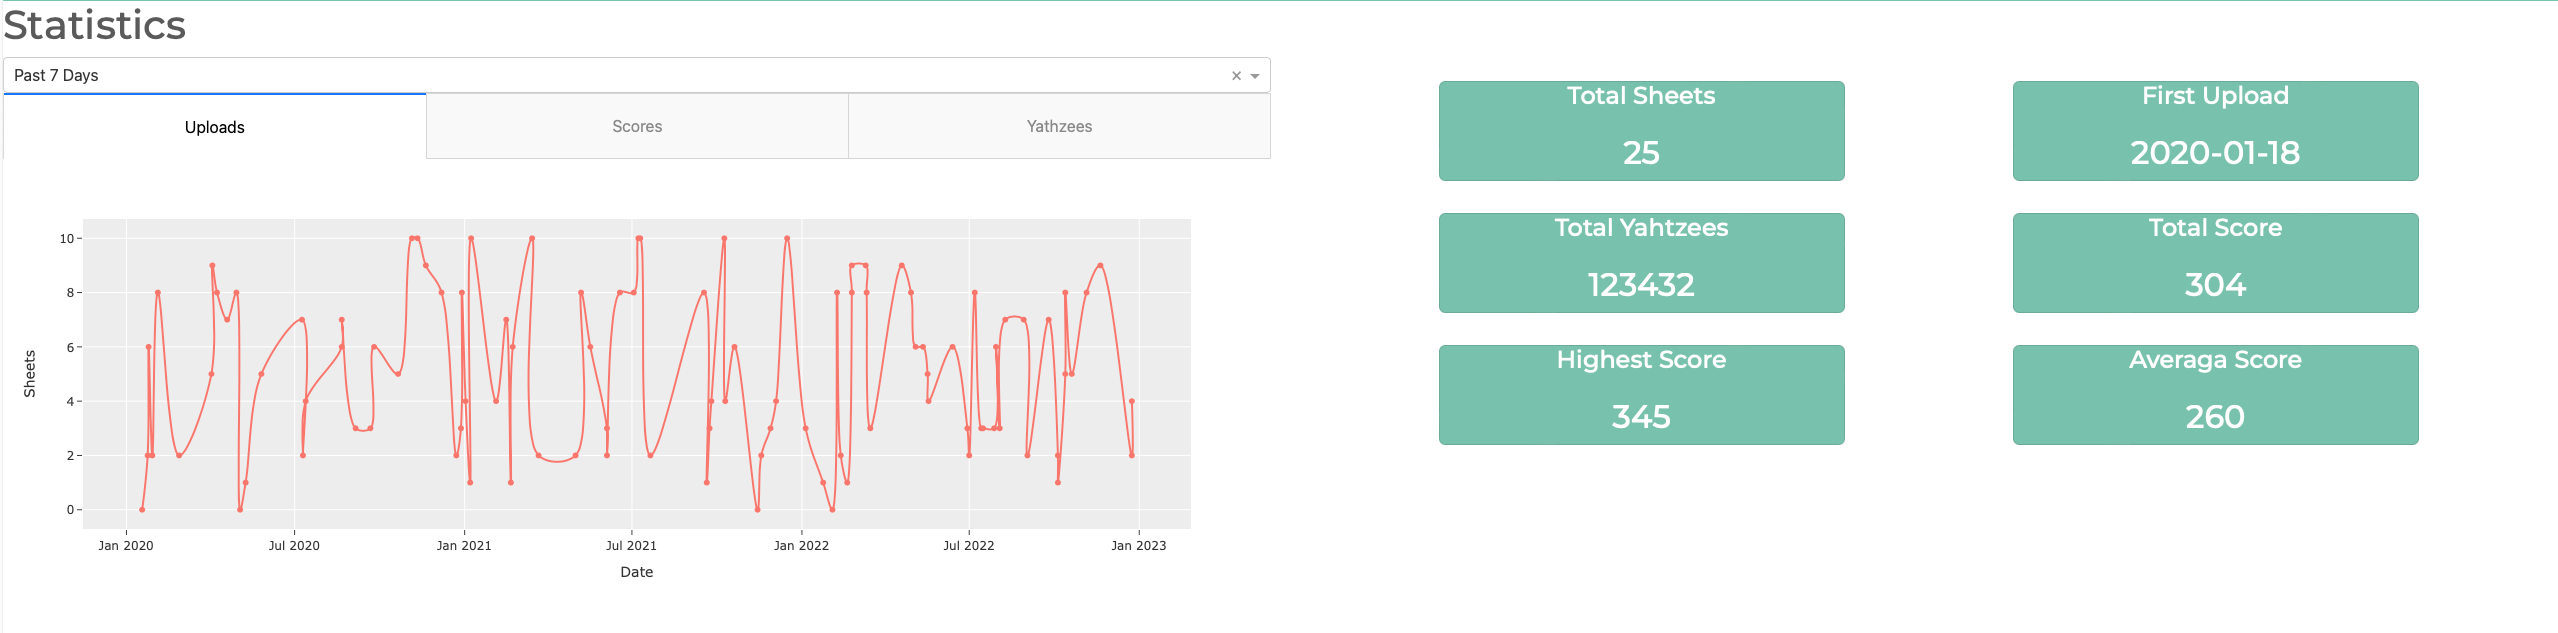
\includegraphics[width=\imgMed]{images/practice/screenshot_dashboard.png}
	\caption{Screenshot vom Dashboard mit Dummy-Daten, selbst erstellt und zugeschnitten}
	\label{fig:dashboard}
\end{figure}

